\documentclass[]{beamer}
\usepackage{color}
\usepackage{listings}
\usepackage{verbatim}
\usepackage{graphicx}
\usepackage{multicol}
\usepackage[utf8]{inputenc}
\usepackage{amsmath}
\usepackage{graphicx}
\usetheme{Madrid}
\title{Bachelor-Thesis}
\subtitle{Simulation of the RoboCup Logistic League with Fawkes and Gazebo for Multi-Robot Coordination Evaluation}
\author {Frederik Zwilling}
\institute{RWTH Aachen}
\date{19.12.2013}
\subject{Multi-Robot Simulation}

\begin{document}
\frame{\titlepage}

%% %Übersicht
%% \begin{frame}
%%   \frametitle{Schedule}
%%   \begin{enumerate}
%%   \item Motivation
%%   \item Background
%%     \begin{enumerate}
%%     \item Logistic League sponsored by Festo
%%     \item Fawkes
%%     %Ros only mentioned besides
%%     \item Gazebo %with advantaged in comperison to other simulators without mentioning them
%%     \end{enumerate}
%%   \item Related Work
%%     \begin{enumerate}
%%     \item Virtual Robotics Challenge
%%     \item RoboCup Simulation Leagues
%%     \item Scene Reconstruction
%%     \item Multi-level Abstraction
%%     \end{enumerate}
%%   \item Approach
%%     \begin{enumerate}
%%     \item Goals-Approaches
%%     \item Architecture (Simulation,Communication,MLA)
%%     \end{enumerate}
%%   \item Implementation
%%     \begin{enumerate}
%%     \item Components
%%     \item Agent Improvements
%%     \end{enumerate}
%%   \item Evaluation
%%     \begin{enumerate}
%%     \item Realism/Limitations
%%     \item Found Problems
%%     \item Statistics
%%     \item Hackathon
%%     \end{enumerate}
%%   \item Future Work
%%   \item Summery
%%     \begin{enumerate}
%%     \item Differences to other siulation, unique features
%%     \end{enumerate}
%%   \end{enumerate}
%% \end{frame}

%Beans
\begin{frame}
  \frametitle{Overview}
  What we have done in this thesis:\\
  \begin{block}{Multi-robot simulation}
    \begin{itemize}
    \item physically and visually realistic 3D environment
    \item \textbf{Domain:} RoboCup Logistic League sponsored by Festo
    \item \textbf{Purpose:} Testing and evaluating to improve our real multi-robot system
    \item \textbf{Focus:} Multi-robot coordination and high level control
    \end{itemize}
  \end{block}
\end{frame}

%First View
\begin{frame}
  \frametitle{First View on the Simulation}

  \begin{figure}
    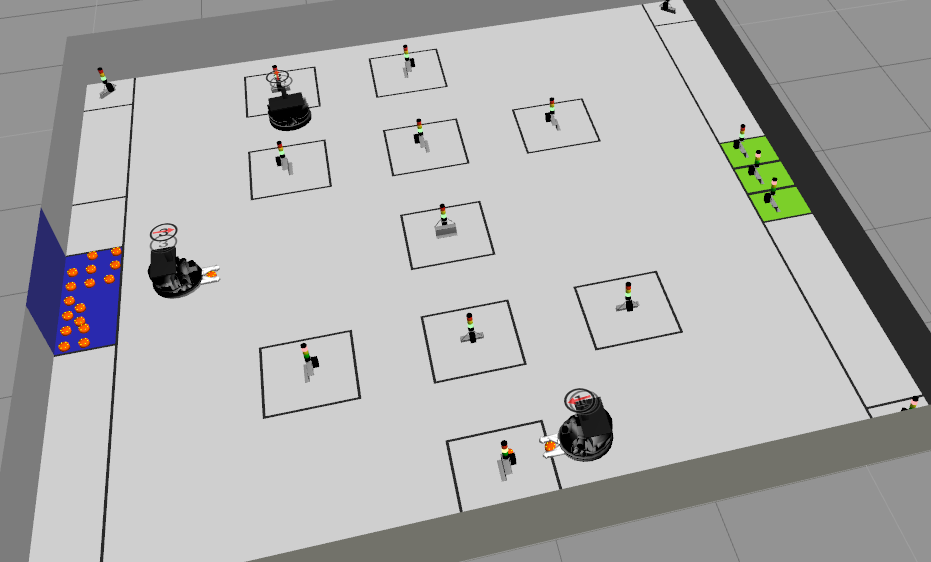
\includegraphics[width=0.7\textwidth]{../pics/sim_working.png}\\
  \end{figure}
\end{frame}

%Schedule
\begin{frame}
  \frametitle{Schedule}
  \begin{enumerate}
  \item Motivation
  \item Background
  \item Related Work
  \item Approach
  \item Implementation
  \item Evaluation
  \item Future Work
  \item Summery
  \end{enumerate}
\end{frame}

%Motivation
\begin{frame}
  \frametitle{Motivation: Multi-Robot Systems and Logistics}
  \begin{multicols}{2}
  Advantages of multi-robot systems:
  \begin{itemize}
  \item Flexibility, parallelism
  \item Heterogenous groups %Division of labour, specializing
  \item Many possible applications %Warehousing, Logistics
  \end{itemize}
  Use in logistics:
  \begin{itemize}
  \item Required parallelism
  \item Individualized workflow
  % Transition: Difficult to test, evaluate
  \end{itemize}
  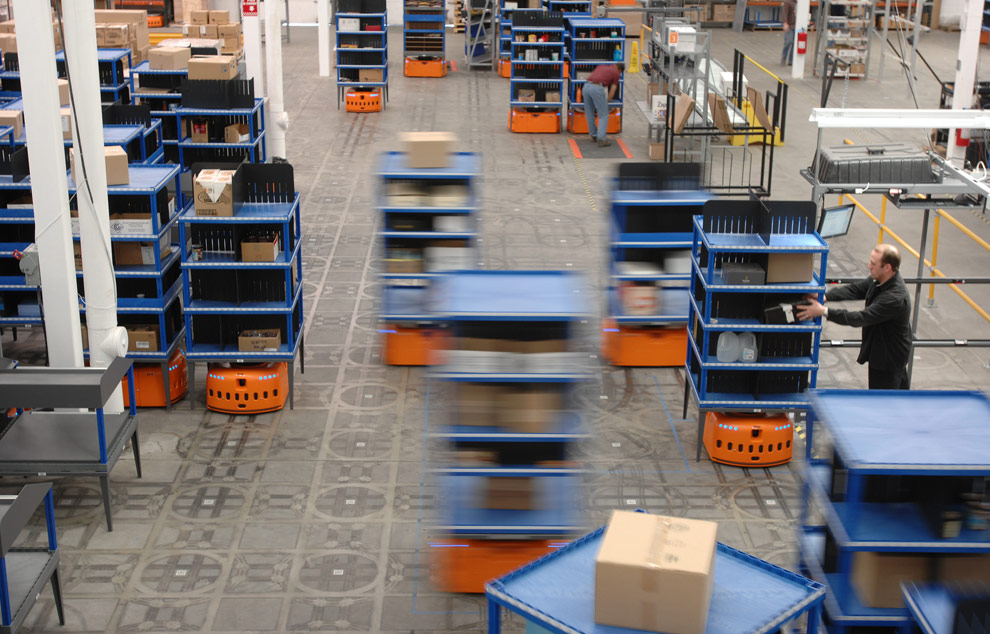
\includegraphics[width=140pt]{../pics/kiva.jpg}
  \end{multicols}
  \textcolor{red}{leave off slide?}
\end{frame}

\begin{frame}
  \frametitle{Motivation: Simulation}
  Advantages of a simulation:
  \begin{itemize}
  \item Possibility to test without real environment and robots
  \item Fast execution of test, automated test runs
  \item Testing on different abstraction levels
  \item Easy comparison of performance with different configurations 
  \item Especially large advantage for multi-robot systems
  \end{itemize}
\end{frame}

%%%% Background %%%%
\begin{frame}
  \frametitle{Logistic League sponsored by Festo (LLSF)}
  \fboxsep=0pt
  \noindent
  \begin{minipage}[]{0.48\linewidth}
    \begin{figure}
      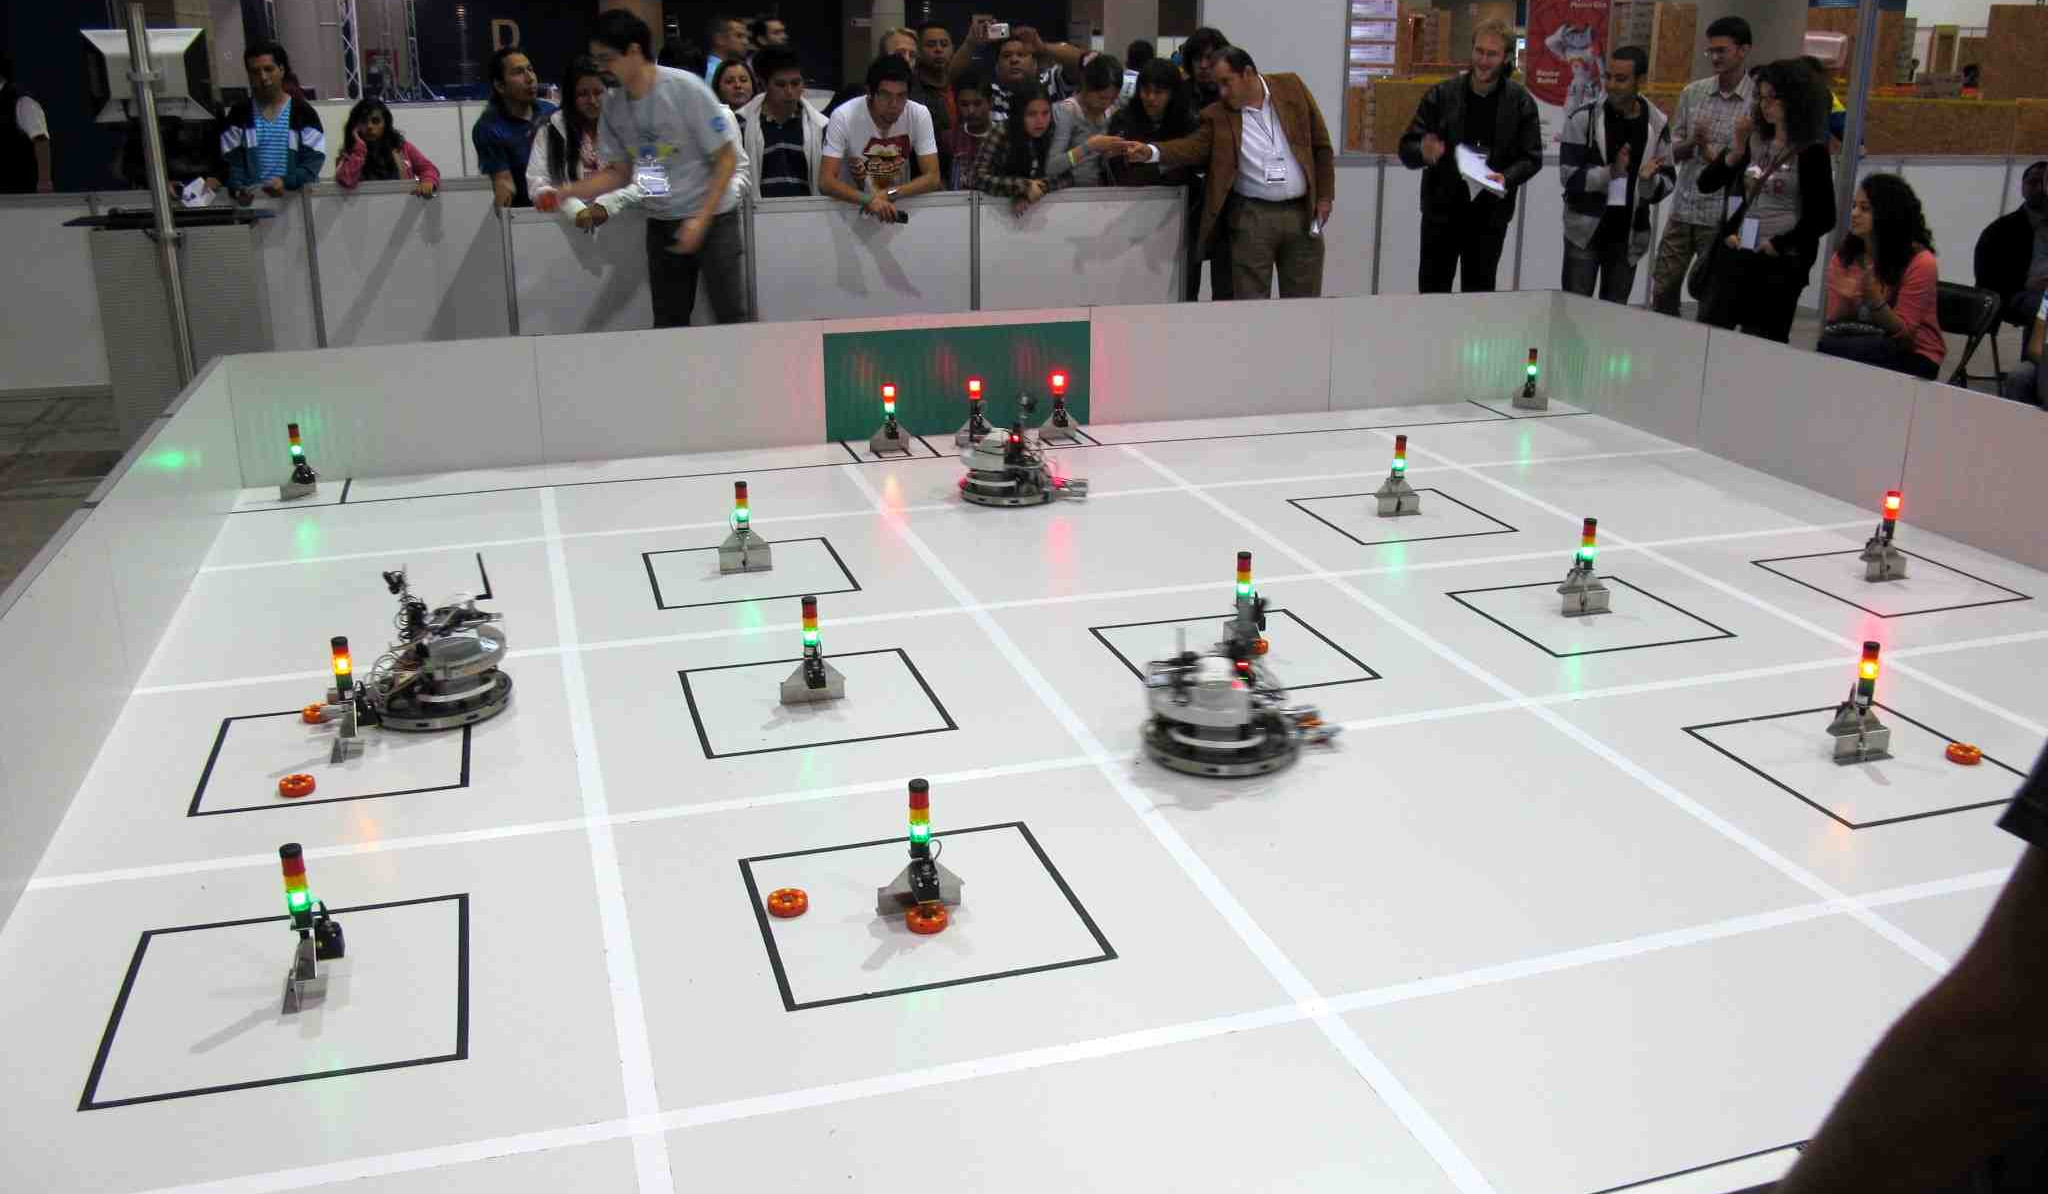
\includegraphics[width=150pt,heigth=120pt]{../pics/llsfLeague.png}\\
    \end{figure}
  \end{minipage}
  \hfill
  \begin{minipage}[]{0.48\linewidth}
    League:
    \begin{itemize}
    \item Part of RoboCup competition
    \item Testbed for logistic robots in a competitive factory automation scenario
    \end{itemize}
    \pause
    Task:
    \begin{itemize}
    \item Produce and deliver products by feeding machines% with resources and semi-finished products
    \item Optimize workflow and performance of the system
    \item Being robust against failure
    \end{itemize}
  \end{minipage}
\end{frame}

\begin{frame}
  \frametitle{Fawkes}
  \begin{multicols}{2}
    \begin{figure}
      \only<1>{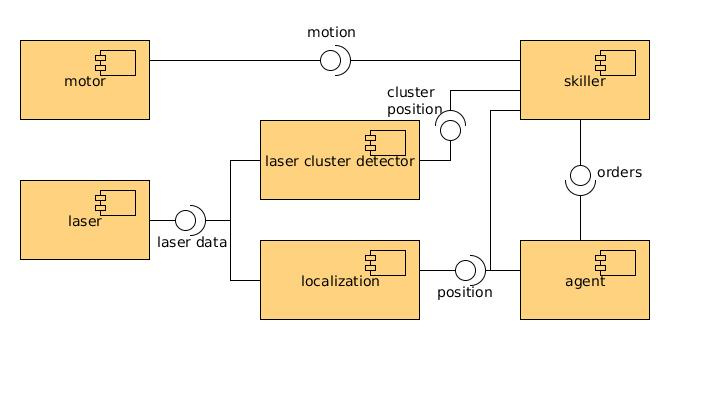
\includegraphics[scale=0.26]{../pics/simplefawkes.jpg}}
      \only<2>{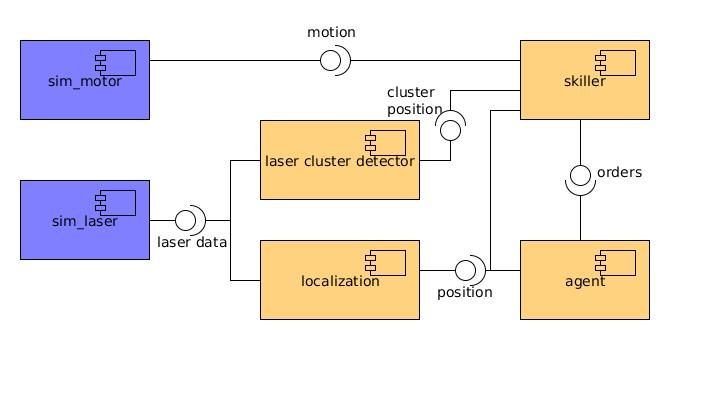
\includegraphics[scale=0.26]{../pics/lowsim.jpg}}
    \end{figure}
    An Open Source robot software framework
    \begin{itemize}
    \item Component-based software design
    \item Components are realized as plugins with multiple threads
    \item Blackboard communication infrastructure
      \pause
    \end{itemize}
  \end{multicols}
  \begin{itemize}
  \item[$\Rightarrow$] Easy exchange of sensor/actuator plugins by simulation plugins
  \end{itemize}
\end{frame}

\begin{frame}
  \frametitle{Gazebo}
  \begin{multicols}{2}
    \begin{figure}
      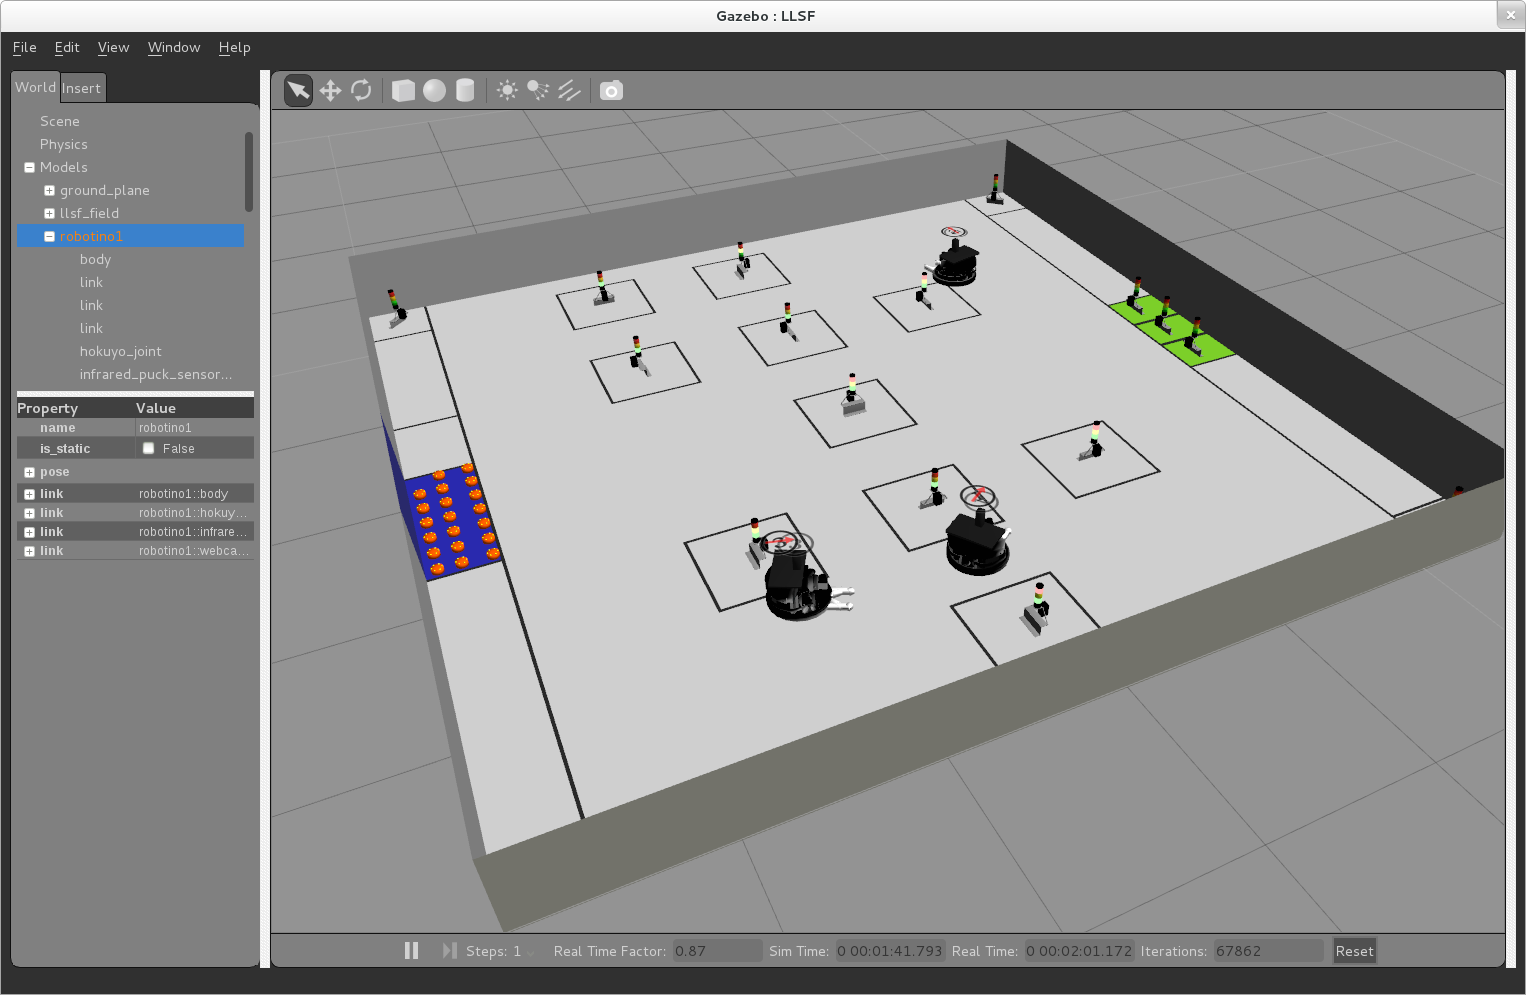
\includegraphics[scale=0.115]{../pics/gazebo_window.png}
    \end{figure}
    An Open Source robot simulator
    \begin{itemize}
    \item Powerful graphics and physics engines %Reflections, Slippery (Odom)
    \item Already supports some robots and sensors (e.g. Hokuyo laser sensor)
    \item Extensive support
    \end{itemize}
  \end{multicols}
\end{frame}

%%%% Related Work %%%%
\begin{frame}
  \frametitle{Related Work}
  \begin{multicols}{2}
    \only<1>{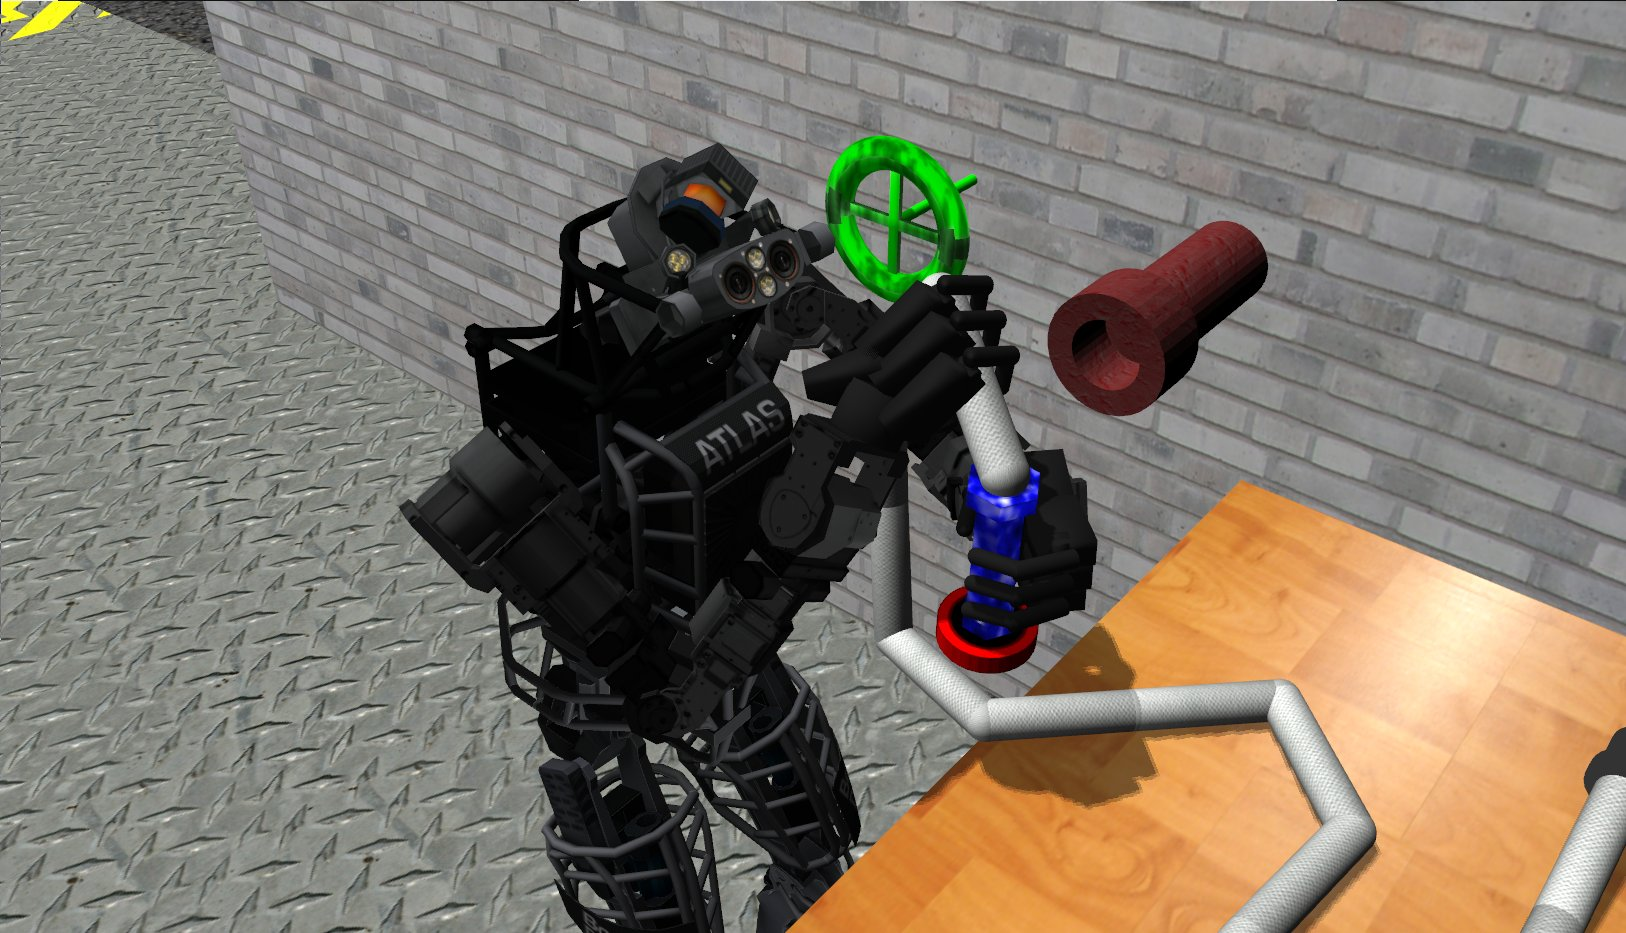
\includegraphics[width=0.52\textwidth,height=0.3\textwidth]{../pics/gazebo.jpg}}
    \only<2>{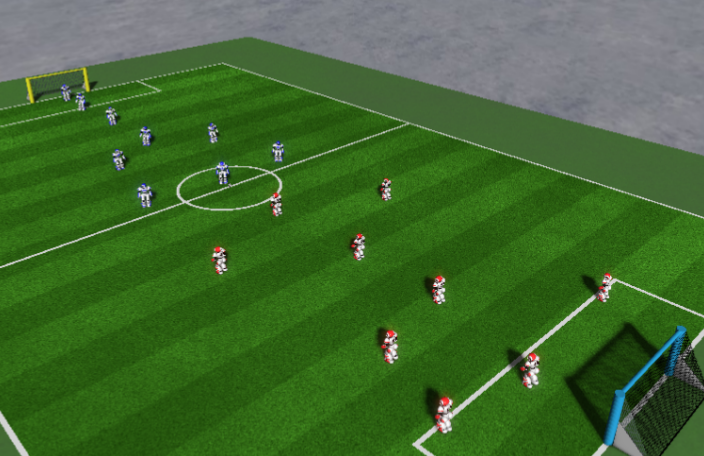
\includegraphics[width=0.52\textwidth,height=0.3\textwidth]{../pics/soccer_simulation_3d.png}}
    \only<3>{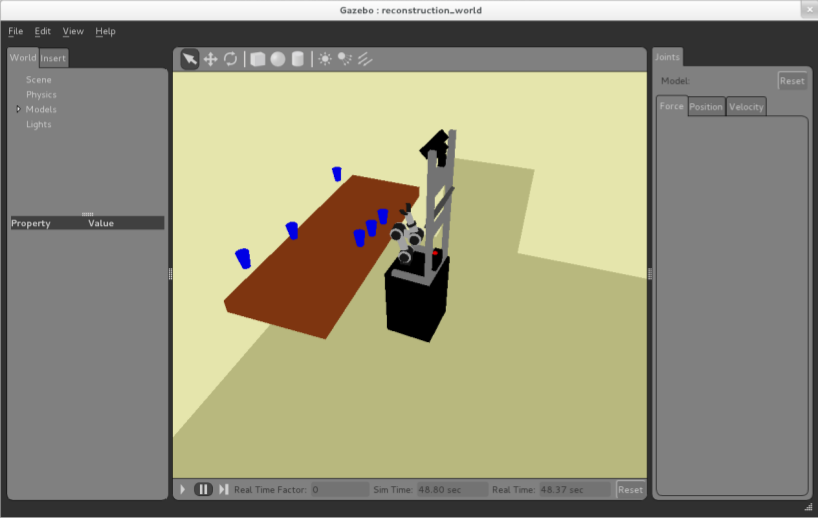
\includegraphics[width=0.52\textwidth,height=0.3\textwidth]{../pics/klingen_sim.png}}
    \only<4>{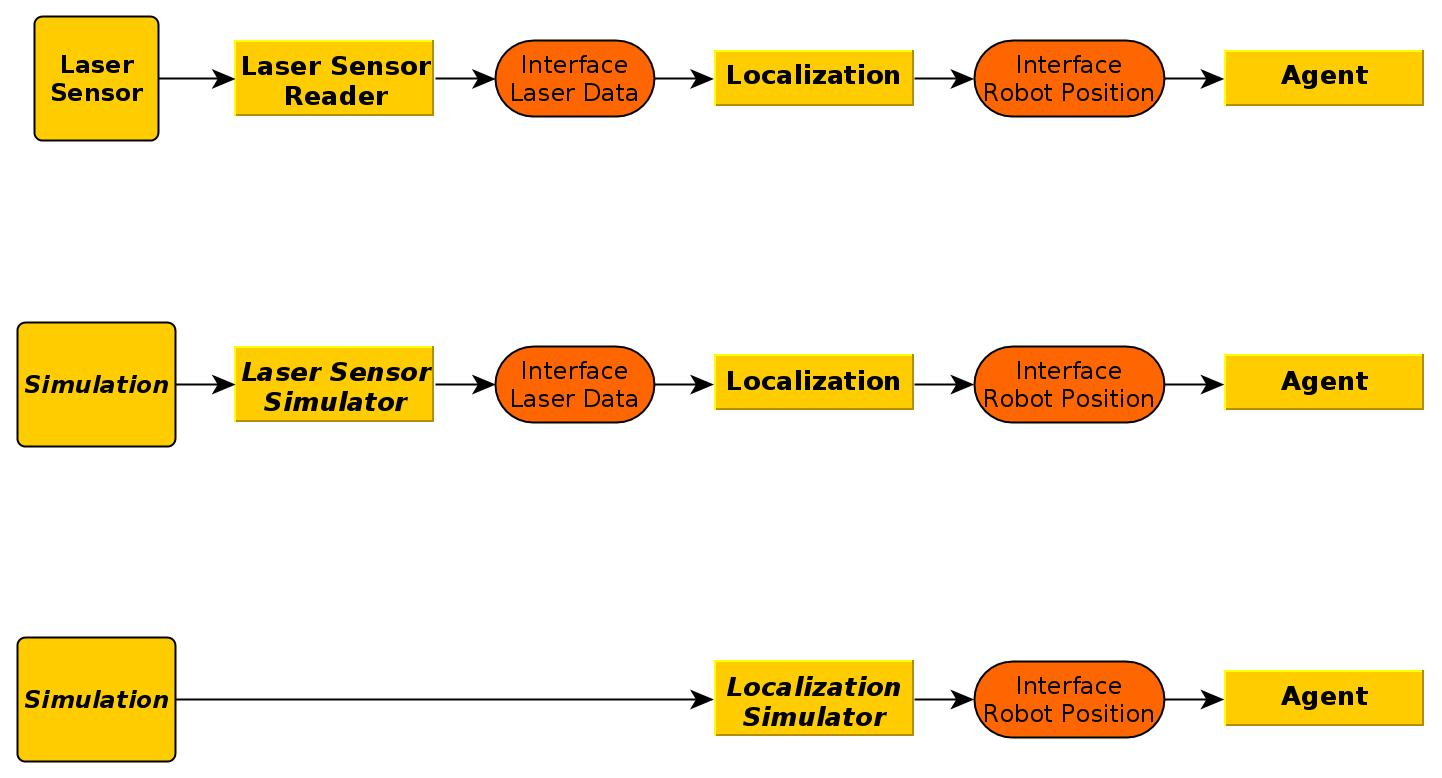
\includegraphics[width=0.52\textwidth,height=0.3\textwidth]{../tabs/mla_complete.jpg}}
    
    \begin{overlayarea}{0.52\textwidth}{.5\textheight}
      \begin{itemize}
      \item Virtual Robotics Challenge
        \pause
      \item RoboCup Simulation Leagues
        \pause
      \item Scene Reconstruction for Fault Analysis
        \pause
      \item Multi-Level Abstraction
      \end{itemize}
    \end{overlayarea}
  \end{multicols}
\end{frame}

%%%% Approach %%%%
\begin{frame}
  \frametitle{Approach}
  \begin{tabular}{p{3.7cm}|p{7.5cm}}
    \hline
    \large{\textbf{Goal}} & \large{\textbf{Approach}}\\
    \hline
    Realistic simulation & Using Gazebo (realistic visuals and physics), \newline Simulating sensors with noise \pause \\ 
    \hline
    Individual testing of high-level components & Mulit-Level Abstraction \pause \\
    \hline
    %Compatibility with original robot software & Replacing plugins, \newline Using the same interfaces \pause\\
    %\hline
    Efficient testing & Startup scripts, \newline Loading different configurations, \newline Visualizing robot belief \pause\\ 
    \hline
    Mulit-robot system evaluation & Scheduling simulation runs, \newline Performance statistics and recording \pause\\    
    \hline
    Expendability & Small and reusable modules \pause\\
    \hline
    Agent improvements & Using three agents, \newline Recycling, \newline Dynamic role change\\
    \hline    
  \end{tabular}
\end{frame}

\begin{frame}
  \frametitle{Architecture: Simulation}
  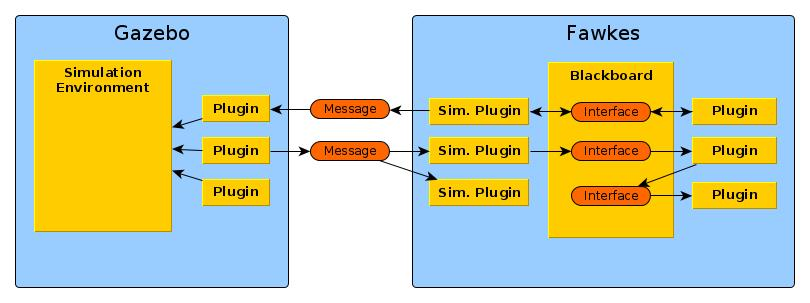
\includegraphics[width=\textwidth]{../tabs/fawkes_gazebo.jpg}
\end{frame}

\begin{frame}
  \frametitle{Architecture: Communication}
  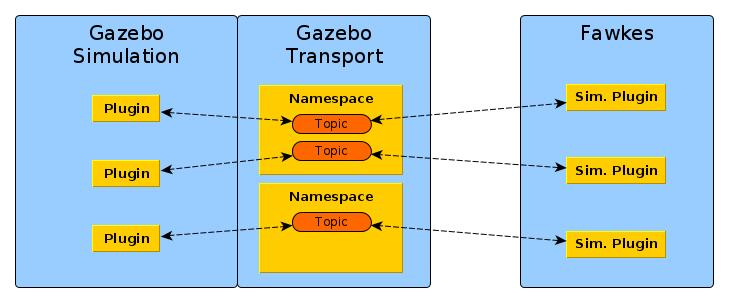
\includegraphics[width=\textwidth]{../tabs/communication.jpg}
\end{frame}

%%%% Implementation %%%%
\begin{frame}
  \frametitle{Implementation}
  ?
\end{frame}

%%%% Evaluation %%%%
\begin{frame}
  \frametitle{Evaluation: Simulation}
  Realism:\\
  %no common measurement => evaluation of components
  \begin{itemize}
  \item LLSF can be simulated realistically
  \item Visualization sufficient for vision tasks %show vision
  \item Reflections and lightening conditions difficult to simulate
  \item Diffucult to find good friction parameters
  \item[$\Rightarrow$] Many real problems can be simulated
  \end{itemize}
\end{frame}


\end{document}
